\section*{C3 inspire}
\label{c3inspire}
\NewsAuthor{Assem Sharma}
\begin{center}

\includegraphics[width=0.8\linewidth]{c3inspire/c3inspire.png}\\
\footnotesize{C3 Inspire [2]}
\end{center}

\textbf{Folgendes Interview habe ich (\href{http://aseemsharma.info/about-me/aseemsharma/}{\textit{Aseem Sharma [1]}}) mit Alim Maherali, dem Gründer von \href{http://c3inspire.com}{\textit{C3 Inspire [2]}}, geführt und habe dadurch einiges gelernt darüber wie man eine Organisation aufbaut und erfolgreich führt basierend auf den \textit{Open-Source} Prinzipien Zusammenarbeit, Vernetzung und Teilen ('collaboration, connections, and sharing')}

Dieser Artikel von  erschien am 17. Dezember 2013 in \href{http://opensource.com/education/13/12/interview-Alim-Maherali-C3-Inspire}{\textit{opensource.com}} unter einer cc-by-sa Lizenz und wurde daher ohne eine Antwort auf Rückfrage abzuwarten von  \textbf{Horst JENS} ins Deutsche übersetzt und republiziert.\\

\begin{center}

\includegraphics[width=0.7\linewidth]{c3inspire/c3inspire_aseemsharma.jpg} \\
\footnotesize{Aseem Sharama. Bildrechte: [1]}
\end{center}

(Beginn der Übersetzung)\\

\subsection*{Open Source als Grundlage von Startup Firmen}
Tatkräftige und motivierte Leute zusammenzubringen um Startups zu 
gründen welche eine positive Auswirkung auf die Gesellschaft haben ist 
ein großartiges, visionäres Unterfangen. Eines davon ist 
\href{http://c3inspire.com/about/}{\textit{C3 Inspire}}, 
dessen Ziel es ist Unternehmer von morgen schon heute 
zusammenzubringen und ihnen eine Plattform und Umgebung zu schaffen auf 
der sie ihre besten Fähigkeiten einbringen können für gemeinsame, 
größere Aufgaben. \\

Im Interview erzählt Alim über eine neue Startup-Businesskultur mit 
einem vorherrschenden Bewusstsein für den Sinn von Zusammenarbeit und 
dem Einsatz von free/libre Open Source Software.


\subsection*{Interview:} 
\textbf{Aseem:} Welche Notwendigkeit in der Welt und im Ausbildungsbereich 
führte Dich dazu C3 Inspire zu gründen ? Welche Prinzipien leiteten 
Dich, welche Mission verfolgst Du mit C3 Inspire ? 
\\ \textbf{Alim:} Ich gründete C3 Inspire wegen der Lücken im Ausbildungswesen die ich 
selbst erfahren hatte als Undergraduate (Bachelor) Student in Waterloo 
Ontario (Kanada).  Ich hatte die einmalige Gelegenheit der erste 
Absolvent eines 2-Studien-Programms zu sein mit Abschlüssen von der 
Universität Waterloo und der Wilfrid Laurier Universität. Als ein 
Student der sowohl eine business school als auch eine technische 
Universität gleichzeitig besucht merkte ich Herausforderungen und 
Fähigkeitslücken denen sich alle Studenten beider Universitäten 
gegenübersehen: 

\begin{center}
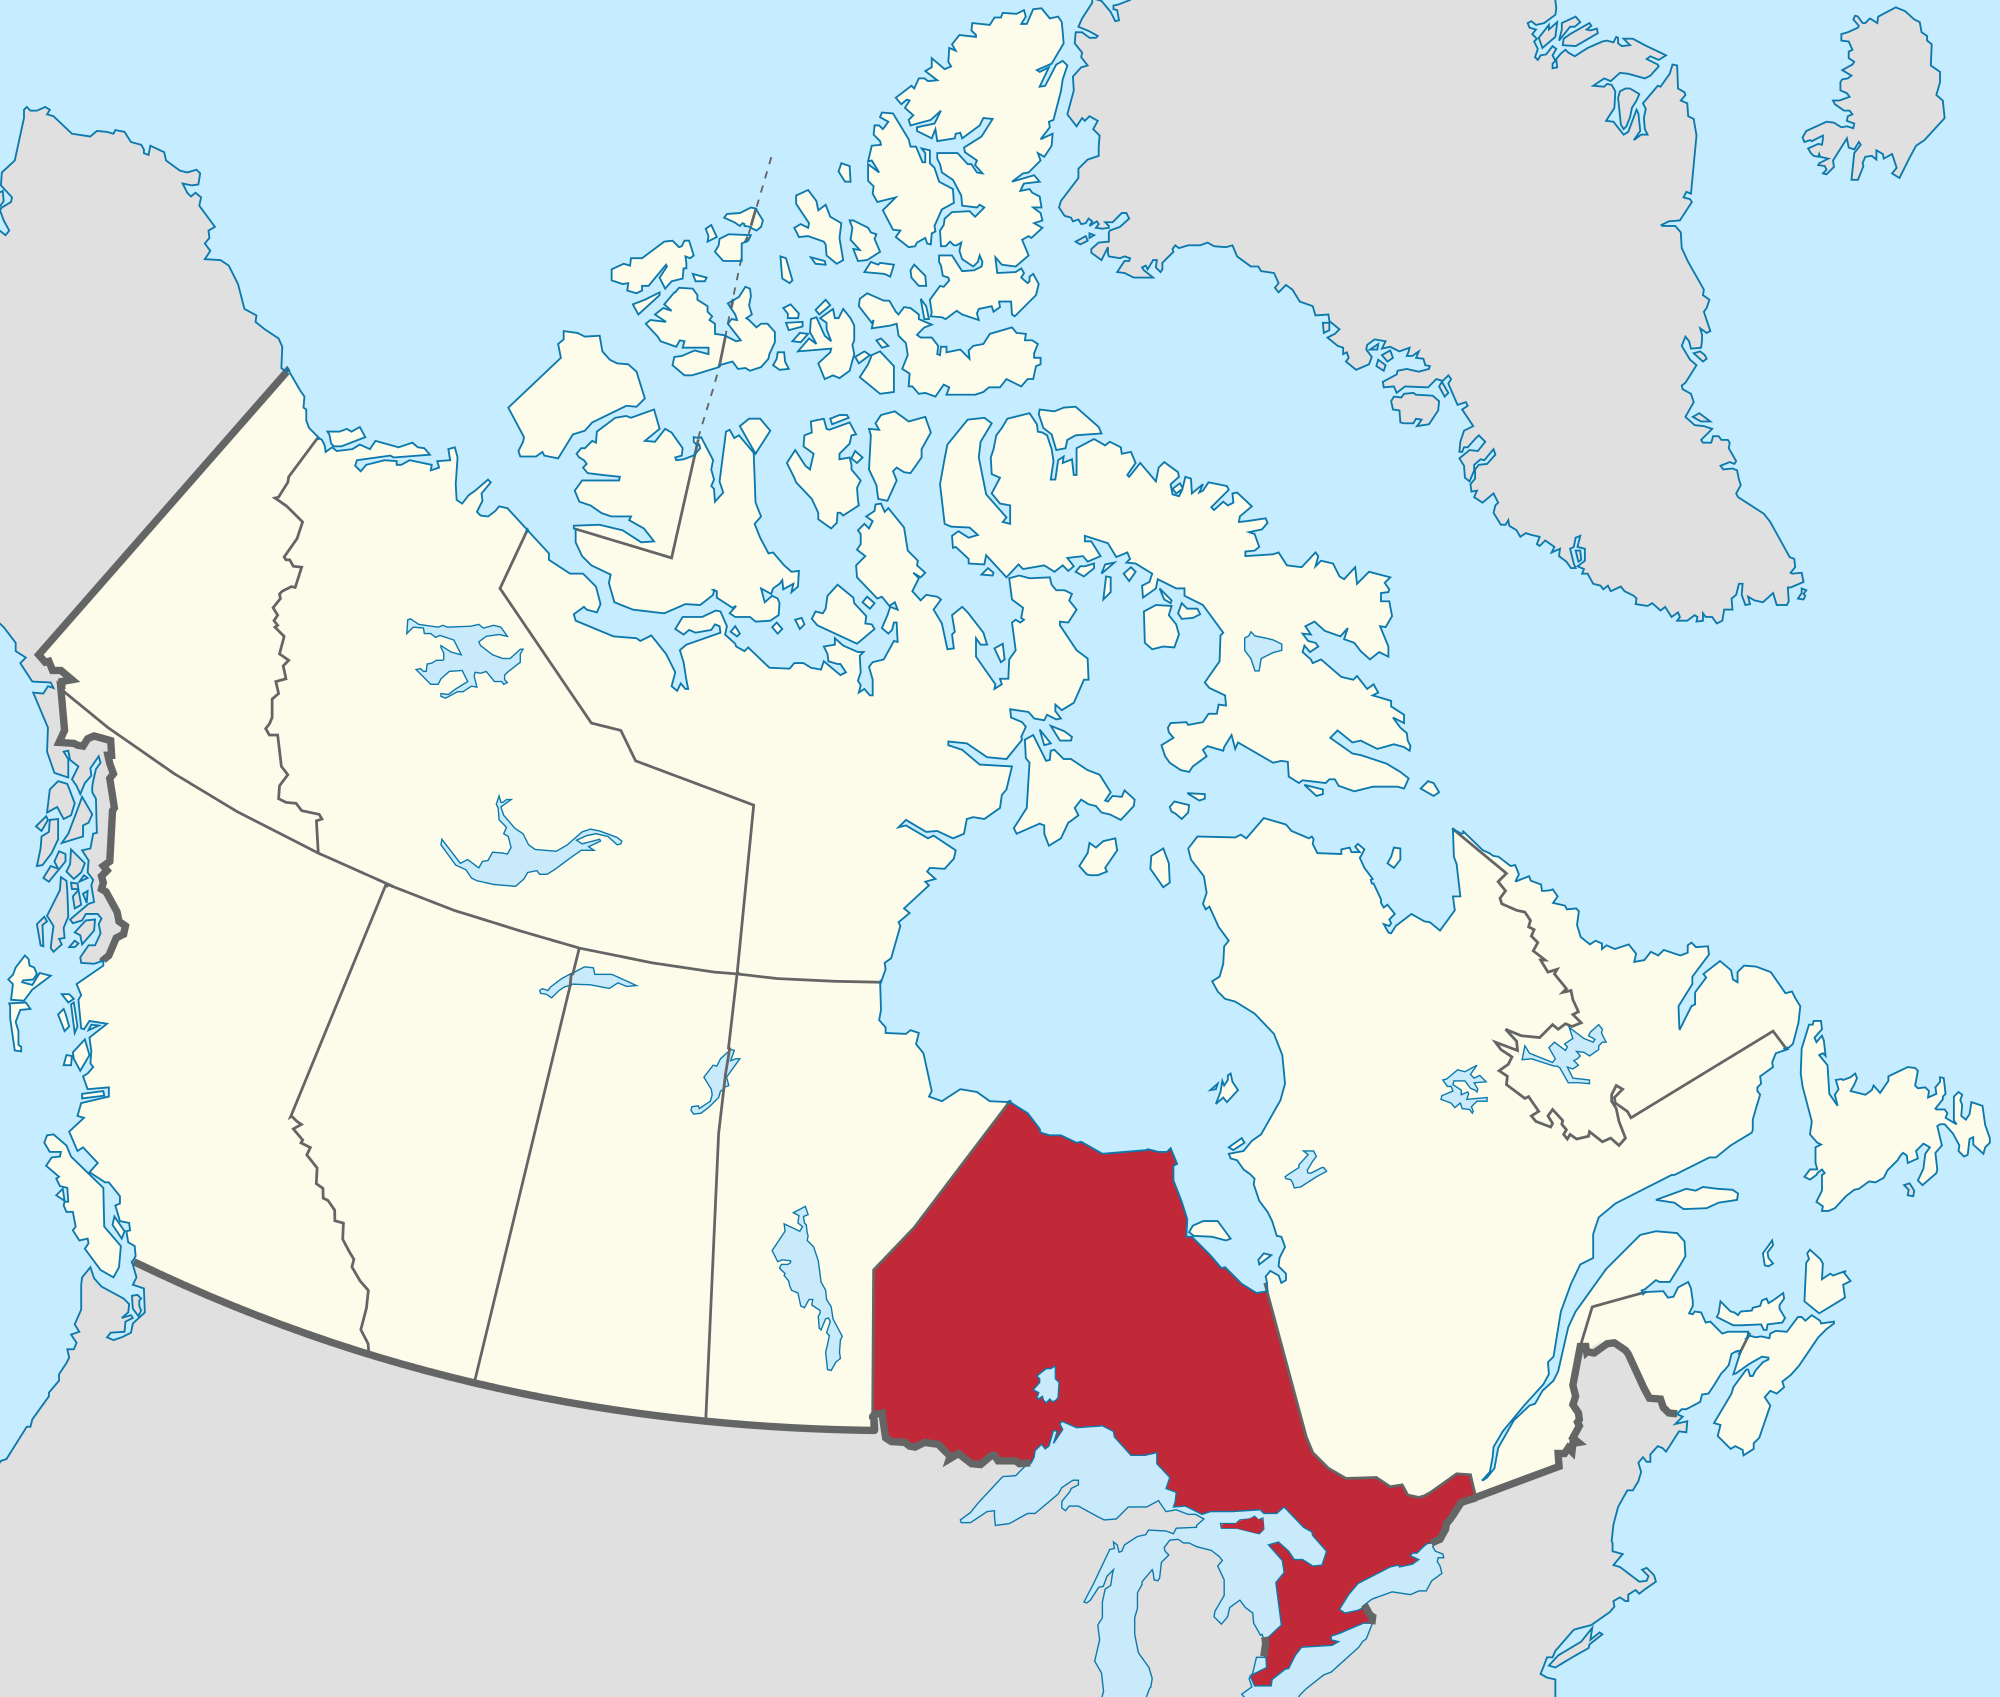
\includegraphics[width=0.7\linewidth]{c3inspire/c3inspire-ontario.png} \\
\footnotesize{Ontario, Kanada. Bildrechte: Tubs [3], \href{https://creativecommons.org/licenses/by-sa/2.5/deed.de}{cc-by-sa}}
\end{center}

Technik-Studenten von der Uni Waterloo fanden es z.B. schwer ihre 
unternehmerischen Ideen zu verwirklichen wegenden fehlendem 
Business-Bereich, z.B. in Finanz und Marketing. 
Daran mangelte es den Studenten an der Wilfried Laurier Uni nicht, die 
konnten unglaublich gut Business-Pläne zusammenstellen aber sie hatten 
Schwierigkeiten damit eine Webseite oder ein eCommerz zu erschaffen 
weil ihnen dazu die technischen Fähigkeiten fehlten. 

C3 Inspire wurde gegründet um Studenten mit unterschiedlichen 
Fähigkeiten und von unterschiedlichen Studienrichtungen zusammen zu 
bringen damit sie sich gegenseitig dabei helfen können ihre Ideen zu 
verwirklichen. 

Ein anderer Grund C3 Inspire zu gründen war der dass sich in jeder der 
beiden Universitäten die besten und scharfsinnigsten Studenten nicht 
miteinander trafen ...erst sehr spät in ihrem Studium. Es gab keine 
Infrastruktur für die besten Studenten einer Uni um zusammen zu kommen. 
Konsequenterweise bedauerten viele Studenten rückblickend dass sie 
sich gegenseitig gerne viel früher besser kennengelernt hätten um 
gemeinsam Projekte zu verwirklichen. 

Schlussendlich: Wirklich jeder dem ich in der Schule über den Weg 
gelaufen bin wollte etwas Sinnvolles (mit seinem Leben) machen ...etwas 
das die Welt zu einem besseren Platz macht. Doch nur einigen wenige 
taten das wirklich. Viele Studenten wollten "später" im Leben etwas 
Sinnvolles tun nachdem sie sich ein paar Jahre lang finanziell 
abgesichert hatten. Leider schaut die Wirklichkeit dass wenn die 
Jahre vergehen, es immer schwieriger wird die Welt zu verändern. Bei 
C3 inspire wollen wir "Soziales Unternehmertum" fördern und anderen 
Studierenden zeigen dass es möglich ist die Welt zu verbessern und 
gleichzeitig eine bezahlte Karriere zu machen. 

Ich war als 'undergraduate student' mit all diesen Herausforderungen 
konfrontiert, und nachdem ich meinen Abschluss gemacht hatte hörte ich 
Jahr für Jahr wie sich die Studenten über die gleichen 
Schwierigkeiten -wie ich sie hatte- beklagten. Nachdem ich die selben 
Klagen von so vielen verschiedenen Studenten gehört hatte dachte ich  
mir, dagegen muss man etwas unternehmen, und damit war die Idee zu C3 
Inspire geboren. Heute ist jeder C3 Event so strukturiert um genau 
diese Probleme anzugehen! 

\paragraph{}
\textbf{Aseem:} Inwieweit verwenden die Startups mit denen du arbeitest freie 
Software und Open Source Technologien bzw. Open Source Methoden ?

\textbf{Alim:} Open Source Lösungen liegen jedem Startup zugrunde mit dem ich 
heute zu tun habe. In Fakt, viele Startups verwenden Open Source 
Technologien für fast alles. Es ist nicht ungewöhnlich für neue 
Firmen dass sie \href{http://wordpress.org/}{\textit{Wordpress}} für ihre Website 
benutzen, \href{http://www.joomla.de/}{\textit{Joomla}} oder \href{https://drupal.org/}{\textit{Drupal}} für ihr 
\href{https://de.wikipedia.org/wiki/Content-Management-System}{\textit{\textbf{CMS}}}, 
\href{https://de.wikipedia.org/wiki/SugarCRM}{\textit{SugarCRM}} für ihr 
\href{https://de.wikipedia.org/wiki/Customer-Relationship-Management}{\textit{\textbf{CRM}}}, und \href{https://de.wikipedia.org/wiki/Trac}{\textit{TRAC}} für Ihr 
\href{https://de.wikipedia.org/wiki/Issue-Tracking-System}{\textit{\textbf{Issue-Tracking} 
System}}.

Unternehmertum bekommt mehr und mehr \href{https://de.wikipedia.org/wiki/Kollaboration}{\textit{kollaborativ}}. Die Tage der 
geheimniskrämerischen Startups welche niemandem erzählen was sie 
vorhaben sind vorbei. (Junge) Unternehmer verstehen dass die Vorteile von 
Zusammenarbeit und Ideen-Austausch bei weitem das Risiko aufwiegen, 
jemand könne ihre Ideen stehlen. Das ganze Unternehmer-Ökosystem 
gleicht sich mehr und mehr dem Open-Source Ökosystem an, wo die 
Menschen wissen dass Zusammenarbeit, etwas beitragen (to contribute),  
allen hilft. Also trägt jeder etwas bei. Es gibt da eine gemeinsame 
Strömung in fast allen unternehmerinschen Aspekten, von 
Gemeinschaftsbüros (shared spaces) zur Standardisierung von 
Risikokapital-Deals.


\paragraph{}
\textbf{Aseem:} Was ist deine Beziehung zur open source Technologie ? Benutzt 
Du freie Software innerhalb Deiner Organisation ? Auch draußen, 'im 
Feld' ?

\textbf{Alim:} Ich sehe freie Software als einen 'Befähiger' für Menschen. 
Freie, Open Source Software erlaubt Menschen finanzielle Hürden zu 
überwinden und gibt ihnen die Chance zum Testen, zum Entdecken und 
zum Erfinden die sie sonst nicht hätten. Nachdem das gesagt ist; ich 
habe enormen Respekt vor kommerzieller Software. Es gibt definitiv 
Situationen wo eine kommerzielle Softwarelösung mehr Sinn macht als 
eine Open Source Lösung, aber beide Arten von Lösungen haben ihren 
Platz und dienen Menschen und Organisationen. C3 Inspire benutzt eine 
breite Auswahl an Open Source Lösungen von Wordpress über GitHub zu 
SugarCRM.

\paragraph{}
\textbf{Aseem:} Welche Rolle spielt Deiner Meinung nach Open Source in der 
Zukunft der Bildung ?

\textbf{Alim:} Open Source Technologien werden weiterhin ein kraftvoller Motor 
für den Bildungssektor sein durch die verstärkte Anwendung von 
\textit{eLearning} Techniken, speziell in Entwicklungsländern. Software wie 
Moodle ist mittlerweile sehr robust und dramatisch positive Resultate 
sind möglich wenn man Lösungen implementiert in Orten wo bisher 
Kosten eine Hürde darstellten. Noch wichtiger: Open Source Sofware ist 
der Bereich wo Erfinder neue Ideen erträumen und austesten. 
Indirekterweise ist dadurch der Einfluss von Open Source Lösungen auf 
Leute im Bildungsbereich außerhalb der traditionellen 
Bildungsinstitutionen ganz schön gewaltig. Meiner Meinung nach werden 
Open Source Lösungen Bildung und Gesellschaft sehr verändern in den 
kommenden Jahren.

\paragraph{}
\textbf{Aseem:} Inwieweit unterscheidet sich C3 Inspire genenüber anderen 
Organisationen und Programmen ?

\textbf{Alim:} C3 Inspire unterscheidet sich in 3 wesentlichen Punkten von 
anderen Organisationen. 

Erstens, C3 Inspire bringt Studenten von 
verschiedensten Universitäten zusammen in Programmen mit 
unterschiedlichen Fähigkeiten. 

Zweitens, C3 Inspire bemüht sich gleichermaßen um die Gründung von 
Sozialen Initiativen wie um die Gründung von (business) Startup's. 

Drittens bringt C3 Inspire Unternehmer, OpenSource Aktivisten und 
erfahrene Profis zusammen um den Studenten zu ermöglichen ihre eigenen 
Ideen zu realisieren. Viele andere Organisationen bringen nur 
Unternehmer zusammen die schon ihre eigenen Ideen haben und deshalb 
nicht sehr auf Zusammenarbeit aus sind. 

Ich glaube es ist die Kombination dieser 3 Elemente die den Studenten 
wirklich hilft ihr Potential zu entfesseln.

\paragraph{}
\textbf{Aseem:} Wie genau arbeitest Du mit Startups ?

\textbf{Alim:} Genau wie in der open Source Community ist Zusammenarbeit auch 
die Grundlage von unseren Werten bei C3 Inspire. Wir machen was wir 
können um andern Startups die mit uns zu tun haben zu helfen und mit 
ihnen zusammen zu arbeiten: Wir haben ein Forum wo Leute sich treffen 
um neue Organisationen gemeinsam zu gründen; wir stellen Startups in 
unserem Blog vor,  wir lassen Startups auf unseren Veranstaltungen 
Vorträge halten. Wir mögen Startups und helfen ihnen gerne.


\subsection*{Fachbegriffe}
~~~\href{https://de.wikipedia.org/wiki/Portal:Freie_Software}{\textbf{Open Source}} Quelloffene (freie) Software. Mit Open Source Prinzipien sind im Artikel der Austauch von Wissen (Sourcecode), Offenheit und Zusammenarbeit gemeint. 

\href{https://de.wikipedia.org/wiki/Content-Management-System}{\textbf{CMS}}: Content Management System, (Inhalts-Management) z.B. ein Wiki (wie Wikipedia) oder ein Blog. 

\href{https://de.wikipedia.org/wiki/Customer-Relationship-Management}{\textbf{CRM}}: Customer Relationship Management System, Kundenbeziehungsvewaltung. Im Prinzip eine Kontakt- bzw. Kundendatenbank.

\href{https://de.wikipedia.org/wiki/Issue-Tracking-System}{\textbf{Issue Tracking}}: auch Trouble-Ticket genannt. Eine Datenbank um Programmierfehler oder Anforderungen an Software zu verwalten. 

\href{https://de.wikipedia.org/wiki/ELearning}{\textbf{e-learning}} elektronisches Lernen: Lernen bei dem moderne Medien (Internet) eingesetzt wird.

\subsection*{Download, Feedback:}
\footnotesize{
Download: Ordner \texttt{c3inspire} \Mundus\ \href{http://spielend-programmieren.at/risjournal/001}{spielend-programmieren.at/risjournal/001}\\
Startseite:\\
\href{http://spielend-programmieren.at/de:ris:001}{spielend-programmieren.at/de:ris:001}\\ 
\Letter\: horst.jens@spielend-programmieren.at}
\normalsize

\subsection*{Lizenz, Quellen:}
\begin{wrapfigure}{l}{2.0cm}

\includegraphics[width=2cm]{c3inspire/ccbysa88x31.png} 
%
\includegraphics[width=2cm]{horst2011mitdoppeltux.jpg}
%\begin{center}
%\footnotesize{Horst JENS}
%\end{center}
\end{wrapfigure}
Dieses Material steht unter der Creative-Commons-Lizenz Namensnennung - Weitergabe unter gleichen Bedingungen 4.0 International. Um eine Kopie dieser Lizenz zu sehen, besuchen Sie \url{http://creativecommons.org/licenses/by-sa/4.0/deed.de}.

\textbf{Quellen:} \\
{[}1{]} \href{http://aseemsharma.info/about-me/aseemsharma/}{aseemsharma.info/about-me} \\
{[}2{]} \href{http://c3inspire.com}{c3inspire.com} \\
{[}3{]} \href{https://commons.wikimedia.org/wiki/User:TUBS}{http://goo.gl/rylcEz} 





